\documentclass[10pt,letterpaper,oneside]{article}
\usepackage[margin=0.76in,headheight=15pt,headsep=18pt,footskip=23pt]{geometry}
\usepackage[T1]{fontenc}
\usepackage[utf8]{inputenc}
% pdfLaTeX-only typography (migrated from fontspec): Libertinus Serif via the
% Type 1 "libertinus" package, Noto Sans as the sans family, DejaVu Sans Mono
% for code.
\usepackage[serif]{libertinus}
\usepackage[sf,nott]{noto}
\usepackage{DejaVuSansMono}
\usepackage{microtype,booktabs,array,tabularx,longtable,multicol,enumitem,needspace,ragged2e}
\usepackage[most]{tcolorbox}
\usepackage{tikz}
\usetikzlibrary{positioning,arrows.meta,shapes.geometric}
\usepackage{xcolor,hyperref,fancyhdr,titlesec,lastpage,graphicx,amsmath,amssymb}
\definecolor{ink}{HTML}{163047}
\definecolor{teal}{HTML}{117D83}
\definecolor{teallight}{HTML}{E9F5F4}
\definecolor{gold}{HTML}{C4923A}
\definecolor{papergray}{HTML}{F3F5F7}
\definecolor{graytext}{HTML}{4E626C}
\definecolor{warn}{HTML}{A5532B}
\definecolor{warnbg}{HTML}{FFF4E9}
\hypersetup{colorlinks=true,linkcolor=teal,urlcolor=teal,pdftitle={Residential Cleaning Operations},pdfauthor={Residential Operations Reference}}
\setlength{\parindent}{0pt}
\setlength{\parskip}{5pt}
\setlength{\emergencystretch}{2em}
\setlist[itemize]{leftmargin=1.5em,itemsep=2pt,topsep=3pt}
\setlist[enumerate]{leftmargin=1.6em,itemsep=3pt,topsep=3pt}
\titleformat{\section}{\sffamily\Large\bfseries\color{ink}}{\thesection}{0.75em}{}
\titleformat{\subsection}{\sffamily\large\bfseries\color{teal}}{\thesubsection}{0.7em}{}
\titleformat{\subsubsection}{\sffamily\normalsize\bfseries\color{ink}}{\thesubsubsection}{0.7em}{}
\titlespacing*{\section}{0pt}{16pt}{7pt}
\titlespacing*{\subsection}{0pt}{12pt}{5pt}
\pagestyle{fancy}\fancyhf{}\fancyhead[L]{\sffamily\small\textcolor{ink}{RESIDENTIAL OPERATIONS / FIELD REFERENCE}}\fancyhead[R]{\sffamily\small\textcolor{teal}{2026 EDITION}}
\fancyfoot[L]{\sffamily\scriptsize\textcolor{graytext}{Controlled reference \textbullet\ Confirm product labels and surface care instructions}}
\fancyfoot[R]{\sffamily\scriptsize\textcolor{ink}{\thepage\ / \pageref{LastPage}}}
\renewcommand{\headrulewidth}{0.35pt}\renewcommand{\footrulewidth}{0pt}
\newtcolorbox{notebox}[1][]{enhanced,breakable,colback=teallight,colframe=teal,boxrule=.55pt,arc=1.5mm,left=9pt,right=9pt,top=7pt,bottom=7pt,#1}
\newtcolorbox{safetybox}[1][]{enhanced,breakable,colback=warnbg,colframe=warn,boxrule=.55pt,arc=1.5mm,left=9pt,right=9pt,top=7pt,bottom=7pt,#1}
\newtcolorbox{plainbox}[1][]{enhanced,breakable,colback=papergray,colframe=papergray,boxrule=.25pt,arc=1.5mm,left=9pt,right=9pt,top=7pt,bottom=7pt,#1}
\newcommand{\kicker}[1]{{\sffamily\bfseries\footnotesize\color{teal}\MakeUppercase{#1}}}
\newcommand{\subtle}[1]{{\color{graytext}\small #1}}
\newcommand{\field}[1]{\textbf{#1}\ \rule{0.22\linewidth}{0.3pt}}
\newcommand{\tick}{\ensuremath{\square}\,}
\newcommand{\task}[1]{\par\noindent\tick #1\par}
\newcommand{\sop}[3]{\Needspace{8\baselineskip}\subsection{#1}\subtle{\textbf{Entry condition:} #2}\par\textbf{Work sequence}\begin{enumerate}#3\end{enumerate}}
\newcommand{\accept}[1]{\begin{notebox}\textbf{Acceptance criteria}\quad #1\end{notebox}}
\newcommand{\sources}[1]{\par{\small\color{graytext}\textit{Basis:} #1}\par}
\newcommand{\coverpage}[4]{%
\pagenumbering{Alph}\thispagestyle{empty}\vspace*{1.13in}\kicker{OPERATIONS SYSTEM / PRACTICAL REFERENCE}\par\vspace{.18in}
{\sffamily\fontsize{28}{34}\selectfont\bfseries\color{ink}#1\par}\vspace{.2in}
{\sffamily\Large\color{teal}#2\par}\vspace{.26in}
{\color{gold}\rule{2.2in}{2.2pt}}\par\vspace{.34in}
\begin{notebox}#3\end{notebox}\vfill
{\sffamily\large\color{ink}\textbf{#4}}\par\vspace{5pt}
{\sffamily\small\color{graytext}Version 1.0 \quad|\quad 10 October 2026 \quad|\quad US residential use}\par
\newpage\pagenumbering{roman}\tableofcontents\newpage\pagenumbering{arabic}}
\newcommand{\refurl}[2]{\href{#2}{#1}}
\newcommand{\smalltable}{\par\small\renewcommand{\arraystretch}{1.24}}
\newcommand{\restorenormalfonttable}{\par\normalsize\renewcommand{\arraystretch}{1}}
\begin{document}
\coverpage{Residential Cleaning\\Operations Guide}{Room-by-room SOPs, safety controls, dependencies and printable schedules}{A practical cleaning system built around \emph{Perfect Maintenance Cleaning} (PMC): plan a route, carry the required tools, work from high to low, finish an area before moving on, and clean floors last. The manual's processes are adapted here with contemporary chemical, surface-care and cross-contamination safeguards.}{Volume 1 of 3 \textbullet\ Standard operating procedures}
\section{Operating model and scope}
\begin{notebox}
\textbf{Three service classes.} \textbf{Daily reset}: dishes, spills, trash, laundry and basic tidying. \textbf{Maintenance / PMC}: repeatable weekly or biweekly kitchen and bathroom cleaning; dusting, vacuuming, and appropriate floor care elsewhere. \textbf{Occasional / deep cleaning}: refrigerator interior, inside oven, window washing, detailed blinds/baseboards, upholstery extraction and similar work. Establish the requested class \emph{before} selecting tasks.\end{notebox}
The source manual is \emph{Speed Cleaning for the Pros: How to Achieve Perfect Maintenance Cleaning}, Jeff Campbell with Debbie Sardone (2011). Its core rules and chapter structure inform the operations sequences below. Proposed checklists, material matrices, safety gates and training criteria are adaptations, not verbatim instructions.\sources{Source manual introduction pp. vii--xi; rules pp. 1--3; kitchen pp. 10--24; bathroom pp. 25--41; dusting pp. 42--56; vacuuming pp. 57--61; refrigerator pp. 62--63; team cleaning pp. 64--67 (printed page numbers).}
\subsection{The operating principles}
\begin{enumerate}
\item \textbf{Move once:} select a starting point, work in a predictable clockwise or continuous path and limit backtracking.
\item \textbf{Carry the right kit:} tools, cloths and approved cleaners should be staged; label each bottle and return it to the same location.
\item \textbf{Follow gravity and access:} high before low, far/back before near/front; avoid dropping debris onto finished surfaces.
\item \textbf{Clean proportionately:} spot-clean an otherwise clean vertical surface, while fully cleaning frequently soiled horizontal surfaces.
\item \textbf{Use minimum effective force:} start with a suitable cloth and mild, compatible product; only escalate after confirming surface and tool safety.
\item \textbf{Manage clean-to-dirty movement:} toilets, contaminated cloths and high-risk zones must not contaminate food-contact or other surfaces.
\item \textbf{Quality before pace:} avoid hurried motions, breakage and rework; measure time only alongside safety and quality.
\end{enumerate}
\begin{safetybox}\textbf{Hierarchy of authority.} Product label and Safety Data Sheet (SDS) \(\rightarrow\) surface / appliance manufacturer's care instructions \(\rightarrow\) applicable public-health or employer rules \(\rightarrow\) this guide \(\rightarrow\) legacy manual examples. If compatibility is uncertain, stop and test an inconspicuous area or obtain permission.\end{safetybox}

\section{Prerequisite-based job order}
\subsection{Whole-home dependency graph}
\begin{center}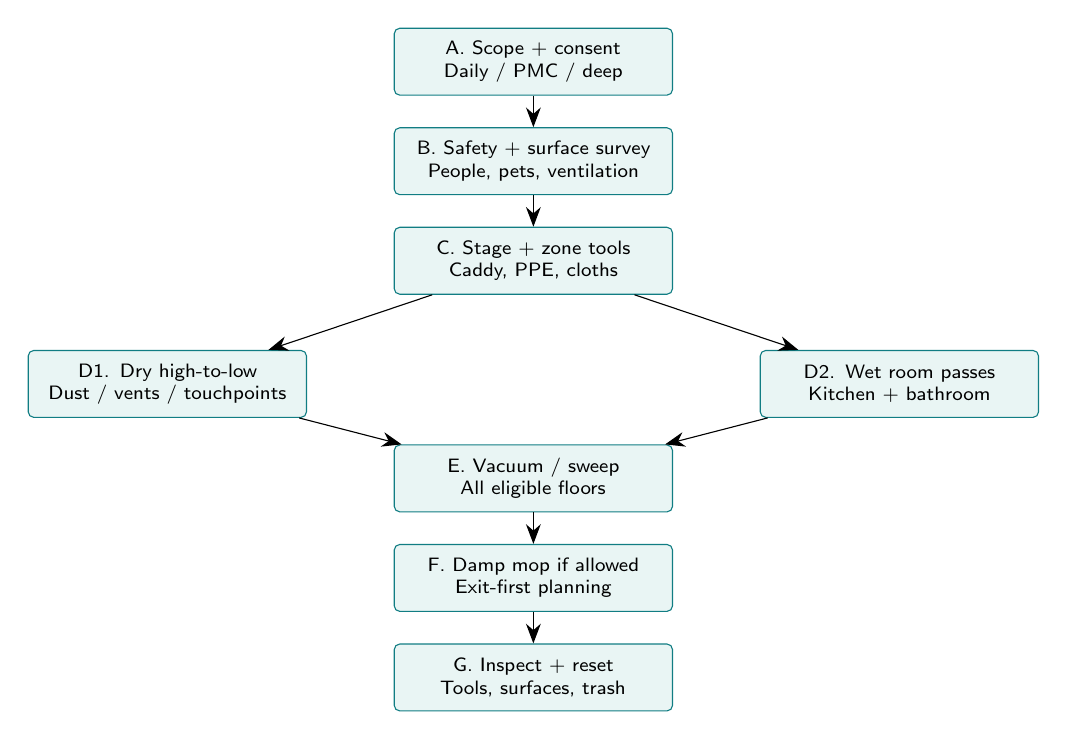
\begin{tikzpicture}[node distance=4mm and 6mm, every node/.style={font=\sffamily\scriptsize}, cell/.style={draw=teal,rounded corners=2pt,fill=teallight,align=center,text width=3.3cm,minimum height=8.5mm}, >={Stealth[length=2.5mm]}]
\node[cell] (a) {A. Scope + consent\\Daily / PMC / deep};
\node[cell,below=of a] (b) {B. Safety + surface survey\\People, pets, ventilation};
\node[cell,below=of b] (c) {C. Stage + zone tools\\Caddy, PPE, cloths};
\node[cell,below left=7mm and 11mm of c] (d) {D1. Dry high-to-low\\Dust / vents / touchpoints};
\node[cell,below right=7mm and 11mm of c] (e) {D2. Wet room passes\\Kitchen + bathroom};
\node[cell,below=19mm of c] (f) {E. Vacuum / sweep\\All eligible floors};
\node[cell,below=of f] (g) {F. Damp mop if allowed\\Exit-first planning};
\node[cell,below=of g] (h) {G. Inspect + reset\\Tools, surfaces, trash};
\draw[->] (a)--(b); \draw[->](b)--(c); \draw[->](c)--(d); \draw[->](c)--(e); \draw[->](d)--(f);\draw[->](e)--(f);\draw[->](f)--(g);\draw[->](g)--(h);
\end{tikzpicture}\end{center}
\textbf{Conditional dependency:} if a refrigerator or oven interior is authorized, start that add-on \emph{before} the normal kitchen circulation so spills and shelf work do not undo already-finished counters. Keep food safe and follow appliance instructions. Bathroom wet-soil removal precedes its dry second pass; vacuuming must follow dusting for each zone.\par
\subsection{Operation gates and stop-work triggers}
\smalltable\begin{longtable}{p{.12\linewidth}p{.31\linewidth}p{.48\linewidth}}\toprule
Gate & Must be true before proceeding & If not true\\\midrule\endhead
G0 & Scope agreed; valuables, fragile items and no-touch zones known & Request instructions; defer unapproved interior appliances, ladders, mold remediation and biohazards.\\
G1 & Surface and finish identified; suitable cleaner selected & Use water/soft dry cloth temporarily or defer; do not guess on natural stone, wood, electronics or coatings.\\
G2 & Gloves, ventilation, label, dilution and any contact time understood & Do not use chemical; find manufacturer guidance.\\
G3 & Clean / toilet tools separated; debris removed before wet cleaning & Restock and re-segregate the kit.\\
G4 & Dry debris controlled; surface can tolerate moisture & Dry vacuum/sweep first; only damp mop if manufacturer permits.\\
G5 & No visible soil, residues, new scratches, wet electrical items or unattended tools & Correct safely, document exclusions and re-inspect.\\\bottomrule\end{longtable}\restorenormalfonttable

\section{Standard setup, zoning and chemical safety}
\subsection{Before entering a room}
\begin{enumerate}
\item Check people and pets; remove trip hazards; establish airflow as the product requires. Never block an exit.
\item Inspect flooring and finishes; photograph existing damage with permission; note loose grout, cracked glass, damaged wires and unstable items.
\item Separate color-coded cloths: \textbf{blue = glass / general dry}; \textbf{green = kitchen}; \textbf{yellow = general bathroom}; \textbf{red = toilet only}. Color mapping is a locally designed convention, not the book's Red/Blue Juice terminology.
\item Assign one cleaner or group of surfaces per cloth face; refold to expose a clean face; replace visibly contaminated cloths. Red-zone cloths never return to counters, taps or mirror work.
\item Carry a neutral all-purpose cleaner, a glass-compatible product only when needed, soft microfiber, non-scratch pad, plastic scraper, soft brush, vacuum tools and a low-moisture mop. Reserve specialized products for special soil and finishes.
\end{enumerate}
\begin{safetybox}\textbf{Chemical prohibitions.} Never mix cleaning chemicals---especially bleach with ammonia, acids/vinegar or toilet cleaners. Never reuse an unlabeled drink container. Do not use bleach as a routine all-purpose bathroom spray; do not invent a universal bleach dilution. If disinfection is warranted, use an EPA-registered product for the surface and organism, follow its exact label concentration and \emph{wet contact time}, and rinse food-contact surfaces when required. Never assume a household cleaner is a disinfectant. Use ventilation, gloves and eye protection when the label or SDS specifies.\end{safetybox}
\sources{Current safety updates: \refurl{CDC household cleaning}{https://www.cdc.gov/hygiene/about/when-and-how-to-clean-and-disinfect-your-home.html}; \refurl{OSHA cleaning chemicals}{https://www.osha.gov/sites/default/files/publications/OSHA3512.pdf}; \refurl{EPA Safer Choice search}{https://www.epa.gov/saferchoice/products}.}
\subsection{Surface compatibility / prohibited shortcuts}
\smalltable\begin{longtable}{p{.23\linewidth}p{.30\linewidth}p{.36\linewidth}}\toprule
Surface & Preferred routine approach & Avoid / escalation\\\midrule\endhead
Sealed laminate counters & Mild compatible detergent; damp microfiber; dry & Powdered abrasives, steel wool, metal scrapers, standing water at seams.\\
Natural stone (marble, limestone, granite) & pH-neutral stone-approved product; soft cloth; rinse/dry if directed & Acids / vinegar; abrasive powders; unknown degreasers; direct bleach unless stone professional approves.\\
Engineered quartz & Manufacturer-approved mild nonabrasive cleaner; soft cloth & Solvents, abrasives, aggressive blades; follow slab-brand guidance.\\
Ceramic / porcelain tile & Neutral tile cleaner, nylon brush for grout; rinse/dry as label directs & Acid on natural-stone tile/grout or adjacent stone; metal scrubbers on glazed finishes.\\
Glass / mirror & Light mist on cloth if edges / backings vulnerable; lint-free dry buff & Excess spray around mirror silvering, outlets or framed art.\\
Chrome / plated hardware & Mild approved cleaner and dry microfiber & Acid descalers left in contact, steel wool, harsh pads.\\
Stainless steel appliances & Finish-compatible gentle cleaner, wipe with grain, dry & Chlorine exposure, harsh abrasion, excessive liquid at controls.\\
Finished hardwood & Dry debris removal; slight damp microfiber if approved; dry promptly & Wet mop, steam, pooled water; use finish-approved cleaner.\\
Laminate flooring & Vacuum/dry mop; minimal dampness only per manufacturer & Soaking joints / wet mopping / steam unless explicitly approved.\\
Luxury vinyl / resilient & Approved neutral cleaner; well-wrung damp mop & Harsh solvents, steam if not approved, abrasive pads.\\
Electronics / touchscreens & Power off as safe; apply device-approved liquid to cloth, not device & Spray into screens, ports, outlets; abrasive cloth.\\
Upholstery / textiles & Vacuum using suitable attachment; inspect care tags & Wet extraction, stain chemicals and saturation without textile-specific approval.\\\bottomrule\end{longtable}\restorenormalfonttable
\sources{Surface advice: \refurl{Natural Stone Institute care}{https://www.naturalstoneinstitute.org/consumers/care/}; \refurl{National Wood Flooring Association}{https://woodfloors.org/maintenance/}; finish-specific products remain subject to manufacturer labels.}

\section{Room-by-room SOPs}
\sop{Kitchen --- PMC standard}{Counters cleared enough to access; burners and appliances cool; approved countertop/finish products selected.}{
\item Place tray near sink; move trash and small mats out of the work line; establish clockwise route from the sink area.
\item Inspect high points and vent/hood exterior for loose dust; clean upper cabinet touchpoints only where soiled; work downward.
\item Wipe backsplash and countertops from rear to front in one zone at a time. Move canisters forward minimally, clean beneath, wipe/dust their outsides as needed, restore original positions.
\item Dust/wipe safe appliance exteriors: refrigerator top, handles and gaskets as accessible; microwave interior is a limited PMC task if agreed. Never immerse or spray appliance controls or outlets.
\item Clean cool cooktop from back to front. Use a non-scratch pad / plastic scraper only when finish-approved; clean knobs carefully without unsafe disassembly.
\item Finish at sink: clean faucet and fixtures, wash bowl with compatible nonabrasive cleaner, rinse per product label, and buff dry. Confirm no product residues remain on food-contact areas.
\item Vacuum/sweep crumbs and edges, then damp mop from the far corner toward the exit using clean covers and correct floor solution. Replace wet covers before they redistribute soil.}
\accept{No loose crumbs, greasy film, fingerprint accumulations, faucet residue or product streaks; appliance controls dry; items reset; floor dry or safely drying.}
\sources{Manual chapter 3 pp. 10--24; product/tool and surface-safety revisions are adaptations.}

\sop{Bathroom --- two-pass PMC method}{No incompatible chemical residues; shower finish, grout, fixtures and slip risk assessed.}{
\item Stage at tub or shower entrance. Remove rugs, trash and movable toiletries while recording placement. Keep a dedicated toilet set in its own compartment.
\item \textbf{Wet pass:} pre-rinse where finish permits; apply compatible bathroom / soap-scum cleaner to shower and tub, observing label dwell time. Brush tile and appropriate grout gently; clean door tracks with a soft detail brush. Rinse fully and dry accessible fixtures.
\item Clean basin interior with appropriate product and non-scratch pad, rinse. Clean \emph{toilet bowl with a dedicated brush} and labeled bowl product; keep the brush isolated.
\item \textbf{Dry/finish pass:} clean vanity, basin exterior, faucet, mirror and cabinet touchpoints, working high to low. Separate toilet exterior cloths from all other cloths. For toilet: tank / flush handle, lid, seat both sides, hinges, bowl exterior, base (cleanest accessible zone to dirtiest).
\item Clean switch plates only with lightly damp cloth (no spray into electrics). Dry vacuum/sweep floor, working around toilet last; mop with a dedicated bathroom cover, moving toward door.
\item Rinse or neutralize only as \emph{required by the product label}; replace items, dispose of waste, wash hands. Persistent widespread mold / damaged caulk = report, not scrub indefinitely.}
\accept{Basin and shower free of soap film; mirror streak-free; toilet clean and dry outside; no cross-use of toilet cloths; no pooled water or chemical odor from overapplication.}
\sources{Manual chapter 4 pp. 25--41; unlike the book's example, bleach application is not a standard final step.}

\sop{Living / family room}{Permission for handling decor and electronics; surfaces identified.}{
\item Start at entry; scan ceiling corners, accessible fixtures, picture-frame tops and shelves; remove dust high to low using capturing microfiber rather than routinely dispersing dust.
\item On each wall segment: dust ledges / horizontal surfaces and objects (without rearranging), wipe visible fingerprints, then dust lower furniture and accessible trim.
\item For electronic screens, follow device instructions and keep spray off hardware. Dust cords and vents without disconnecting devices.
\item Vacuum upholstery and under movable cushions only if included; move light furniture only if safe and approved; return objects to original positions.
\item Vacuum carpets or dry clean hard floor once dusting has finished. Damp mop hard floors only where finish permits.}
\accept{No visible dust on high-touch ledges, tables, accessible frames or electronics; no disturbed decor; floor debris removed.}
\sources{Manual dusting pp. 42--56 and vacuuming pp. 57--61.}

\sop{Bedrooms and closets (accessible portions)}{Bedding / laundry scope known; private storage exclusions agreed.}{
\item Top-to-bottom inspection of ceiling corners, blinds, shelf edges, frames and headboard; use microfiber to capture dust.
\item Lightly wipe reachable furniture tops, drawer pulls and switches; do not open drawers, handle valuables or reorganize personal items without authorization.
\item Make bed or change linens only if specifically in the agreed service class; place used linens directly in laundry container.
\item Vacuum under reachable bed edges with the correct head and without pulling cords / furniture; clean visible floor last.}
\accept{Accessible surfaces dust-free, items in place, no dust piles under reachable edges, permitted floor care complete.}
\sources{Manual general dusting and vacuuming chapters; bedding / privacy instructions are added operational controls.}

\sop{Entry, hallway and stairs}{Shoes, mats and trip hazards addressed; suitable carpet / hard-surface attachments available.}{
\item High dusting along corners, rails, frame tops and accessible ledges.
\item Spot-clean handrails, switches and door handles with finish-compatible product.
\item Vacuum stairs from a stable position using a stair-safe tool; control cord to prevent trips. Never stretch or stand on stairs while operating an unstable appliance.
\item Vacuum/sweep edges, remove mats for cleaning if authorized, and damp mop appropriate hard floors toward the exit.}
\accept{Rails and touchpoints clean; stair treads free of loose debris; runners flat and not left as trip hazards.}
\sources{Manual dusting / vacuuming framework; stair cord-risk additions are safety adaptations.}

\sop{Laundry / utility / mudroom}{Appliances off or safe to wipe; no electrical or water leaks; owner has specified laundry scope.}{
\item Dust reachable high surfaces, shelves and exhaust register covers (do not dismantle or open live equipment).
\item Wipe appliance exteriors and handles with a nearly dry microfiber; keep liquids away from electrical panels.
\item Wipe sink / folding counter and reachable shelving; spot-clean doors / hooks / baskets if necessary.
\item Remove lint from \emph{dryer lint screen after each load} when in scope; duct cleaning or appliance maintenance is a separate service.
\item Sweep/vacuum and damp mop allowed floor; return laundry products upright.}
\accept{No loose lint or grit on exposed surfaces; controls dry; detergent bottles secure; floor not slippery.}
\sources{Extension of manual's kitchen/dusting method; laundry-room content is new, not a source-manual chapter.}

\sop{Interior refrigerator --- authorized deep-clean add-on}{Customer authorizes; foods safe to move; appliance manual checked; food-contact cleaner approved.}{
\item Schedule \emph{before routine kitchen PMC}; prepare a clean staging area and handle perishables promptly. Discard food only with explicit permission.
\item Work shelf by shelf from top to bottom. Move or remove minimum items, supporting glass shelves; allow cold glass to warm before applying temperature-changing water.
\item Wash removable bins in accordance with manufacturer instructions; use food-contact-safe products, required rinse and thorough dry. Clean door gaskets with a soft brush.
\item Wipe residual moisture and restore food in correct places; leave temperature setting unchanged. Close promptly and confirm door seal.
\item Resume normal kitchen pass, ending with appliance exterior.}
\accept{No visible spills or cleaner residue; bins dry; food returned; door seals and temperature controls undisturbed.}
\sources{Manual refrigerator pp. 62--63 identifies this as \emph{outside} maintenance cleaning; food-contact / temperature controls are added.}

\section{Staffing, pacing and quality assurance}
\smalltable\begin{tabularx}{\linewidth}{p{.17\linewidth}X X}\toprule
Crew & Initial parallel roles & Finish-together adjustment\\\midrule
1 person & Kitchen \(\to\) bathroom \(\to\) dry rooms \(\to\) floors (sequence can adapt to drying and travel) & Avoid backtracking; batch dry rooms before vacuuming.\\
2 people & Kitchen person; bathroom person, then switch to dusting/vacuuming when their area is released & Start the longest non-shared job early; avoid two staff crowding the same room.\\
3 people & Kitchen; bathroom; duster / team lead & Team lead assigns vacuuming to completed/dusted zones; redistribute short final tasks.\\\bottomrule\end{tabularx}\restorenormalfonttable
\textbf{Acceptance inspection:} at every room boundary, visually inspect at standing and normal seated height; check touchpoints, rim edges, corners, residue, odor, water and surface damage. Run a ten-point final audit: (1) scopes completed, (2) color segregation maintained, (3) no visible high dust, (4) no soil on horizontal surfaces, (5) glass clear, (6) fittings dry, (7) floors free of grit, (8) nothing relocated, (9) no chemical/tool left, (10) deviations recorded. \par
\textbf{Performance metrics}: rework rate = rooms needing correction / rooms inspected; first-pass quality = rooms passing first inspection / rooms inspected; \(\text{time efficiency}=\frac{\text{accepted rooms}}{\text{person-hours}}\). Use metrics for coaching, never to incentivize rushed chemical use.\sources{Team planning from manual pp. 64--67; audit criteria and metrics newly designed.}

\section{Schedule and frequency policy}
Frequency is a planning baseline, not a universal hygiene mandate. Increase where usage, pets, allergies, illness, food handling or visible soil requires; reduce for unused guest rooms without omitting inspections. For infection concerns, follow CDC advice and the disinfectant label, not a fixed schedule alone.
\subsection{Daily / after-use reset}
\begin{itemize}
\item Kitchen: wipe food spills and high-use counters; dishes, sink, food-contact tools; spot sweep.
\item Bathroom: dry shower walls with squeegee if suitable; wipe fresh splashes; ventilate; keep toilet visibly clean.
\item Living / bedrooms: put away clutter; spot-treat spills; keep high-touch spots clean; manage laundry and trash.
\item Entry: remove grit and wet footwear; dry any standing water.
\end{itemize}
\subsection{Weekly / biweekly PMC cycle}
Clean bathroom fixtures and high-use shower surfaces; kitchen exterior surfaces and sink; dust reachable rooms; vacuum upholstery / carpets / edges as needed; mop approved hard floors; empty waste; perform acceptance checklist. High-use kitchens and bathrooms usually need a weekly pass even when a full-home service occurs biweekly.
\subsection{Monthly detail rotation}
\begin{itemize}
\item Week 1: reachable door edges and fingerprints, cabinet faces, lower trim; check residue beneath small appliances.
\item Week 2: accessible shutters/blinds / vent covers; dust lamp shades as material permits.
\item Week 3: refrigerator gaskets / exterior vents and accessible drawers; inspect, not automatically empty, interior.
\item Week 4: high and low dust traps, behind safely movable light furniture, mop-pad condition and vacuum filter/belt per instructions.
\end{itemize}
\subsection{Seasonal / quarterly scope}
Schedule separately if approved: refrigerator / freezer interior; oven interior; wash accessible windows; clean blinds / baseboards in detail; rotate upholstery; declutter / storage; evaluate grout and caulk for repair rather than concealment; clean dryer duct via suitable service; check filter and equipment maintenance. Service scope, physical access and surface compatibility control inclusion.

\section{Printable checklists}
\newpage\subsection*{FORM O-01 / Preflight and safety release}
\field{Home / area:} \qquad \textbf{Date:} \rule{1.2in}{.3pt} \qquad \textbf{Cleaner:} \rule{1in}{.3pt}
\begin{plainbox}
\task{Agreed scope: \(\square\) daily \(\square\) PMC \(\square\) deep add-on; exclusions documented}
\task{Pets / people / access restrictions accounted for}
\task{Floor finishes, stone, wood, painted surfaces and special items identified}
\task{Existing damage, electrical hazards, unstable items and wet slips checked}
\task{Ventilation, PPE, product labels and any SDS verified}
\task{Sprayers labeled; no unsafe decanted or mixed chemicals}
\task{Kitchen, general bathroom and toilet cloths segregated}
\task{Vacuum, mop covers and soft brushes inspected; replacements staged}
\task{Refrigerator/oven/window interiors authorized, if applicable}
\task{Exit path, cords and equipment staging safe}
\end{plainbox}
\textbf{Exceptions / stop-work notes:}\par\rule{\linewidth}{.3pt}\par\vspace{13pt}\rule{\linewidth}{.3pt}
\textbf{Approved by / time:} \rule{.68\linewidth}{.3pt}
\newpage\subsection*{FORM O-02 / Room completion card}
\textbf{Room:} \rule{1.5in}{.3pt}\quad\textbf{Type:} \rule{1.5in}{.3pt}\quad\textbf{Start / end:} \rule{1.1in}{.3pt}
\begin{plainbox}
\task{Scope and finish checked; correct cloth color / product selected}
\task{Trash / loose mats / agreed clutter positioned}
\task{Ceiling corners / accessible highs / fixtures checked}
\task{All horizontal ledges and touchpoints addressed}
\task{Soiled vertical areas spot-cleaned; items returned}
\task{Room-specific wet fixtures completed and residues rinsed if needed}
\task{Toilet zone / food zone cross-contamination prevented}
\task{Floor dry debris removed and approved damp care completed}
\task{No standing water, streaks, scratches, chemical residues or debris}
\task{Tools removed, waste taken, walkthrough completed}
\end{plainbox}
\textbf{QC pass:} \(\square\) first pass \(\square\) corrected \(\square\) deferred\quad \textbf{Inspector:} \rule{1.7in}{.3pt}\par\vspace{11pt}\textbf{Deferred work and reason:}\par\rule{\linewidth}{.3pt}\par\vspace{9pt}\rule{\linewidth}{.3pt}
\newpage\subsection*{FORM O-03 / Weekly cleaning route}
\textbf{Week of:} \rule{1.8in}{.3pt}\qquad \textbf{Team:} \rule{2.4in}{.3pt}\par\medskip
\begin{tabularx}{\linewidth}{p{.26\linewidth}X p{.21\linewidth}}\toprule Area & Key scope & Done / notes\\\midrule
Kitchen & Cabinet handles, counters, backsplash, appliances, sink, floor & \(\square\) \\
Primary bathroom & Shower/tub, basin, toilet, mirror, floor & \(\square\) \\
Additional bathroom & Soil-based wet pass; sink, toilet, floor & \(\square\) \\
Living / family & Dust, upholstery if agreed, vacuum/floor & \(\square\) \\
Bedrooms & Dust, approved bed service, floor & \(\square\) \\
Hall / stairs / entry & Rails, switches, corners, mats, treads & \(\square\) \\
Laundry / utility & Surfaces, lint screen if included, floor & \(\square\) \\
Detail rotation & Monthly selected area / item & \(\square\) \\
Final audit & Streaks, contamination, residue, reset, tools & \(\square\) \\
\bottomrule\end{tabularx}
\vspace{14pt}\textbf{Observed issues / additional authorization:}\par\vspace{14pt}\rule{\linewidth}{.3pt}
\newpage\subsection*{FORM O-04 / Seasonal service authorization}
\textbf{Date:} \rule{2in}{.3pt}\quad\textbf{Home:} \rule{2.5in}{.3pt}
\begin{plainbox}
\task{Refrigerator / freezer interior; food-handling plan confirmed}
\task{Oven interior per appliance manufacturer / cool-down procedure}
\task{Interior windows / tracks reachable without unsafe ladders}
\task{Blinds / baseboards / upper trim detailed, with finish-compatibility approval}
\task{Upholstery / carpets: approved tools and textile tags checked}
\task{Grout / caulk maintenance defects logged for repair}
\task{Hardwood / stone / specialty surfaces: approved product confirmed}
\task{Equipment: filters, mop covers, vacuum and brushes inspected}
\task{Resident approval for moving / discarding belongings recorded}
\end{plainbox}
\textbf{Special exclusions / planned hours:}\par\rule{\linewidth}{.3pt}\vspace{18pt}\par\rule{\linewidth}{.3pt}
\section{References and lineage}
\begin{enumerate}
\item Campbell, Jeff, with Debbie Sardone. \emph{Speed Cleaning for the Pros: How to Achieve Perfect Maintenance Cleaning}. Self-published, 2011. User-supplied 82-page PDF; consult original chapters for historical PMC terminology and detailed original examples.
\item \refurl{CDC --- When and How to Clean and Disinfect Your Home (2025)}{https://www.cdc.gov/hygiene/about/when-and-how-to-clean-and-disinfect-your-home.html}.
\item \refurl{OSHA --- Protecting Workers Who Use Cleaning Chemicals}{https://www.osha.gov/sites/default/files/publications/OSHA3512.pdf}.
\item \refurl{EPA --- Search Safer Choice-Certified Products}{https://www.epa.gov/saferchoice/products}.
\item \refurl{Natural Stone Institute --- Care and Cleaning}{https://www.naturalstoneinstitute.org/consumers/care/}.
\item \refurl{National Wood Flooring Association --- Maintenance}{https://woodfloors.org/maintenance/}.
\end{enumerate}
\begin{notebox}\textbf{Source/adaptation distinction.} PMC's sequential routing, tool staging, kitchen process, bathroom two-pass concept, dusting / vacuuming roles and team balancing derive from the 2011 manual. Modernized chemical restrictions, surface matrix, color-coded zones, quality metrics, floor-moisture controls, schedules and forms are additions. The guide is not an assertion that the 2011 manual endorses these updates.\end{notebox}
\end{document}
